\documentclass[11.5pt]{article}

\usepackage{amssymb, amsmath, amsthm, amsfonts, eurosym, geometry, ulem, graphicx, caption, color, setspace, footmisc, pdflscape, array, todonotes, subfig, adjustbox, booktabs, pdfpages, siunitx, setspace, multirow, tikz, appendix}

\usepackage[flushleft]{threeparttable}
%\usepackage{hyperref}
\usepackage{natbib}
\bibliographystyle{plainnat}
%\usepackage[round]{natbib}
\usepackage[applemac]{inputenc}
\usepackage{hyperref}
%\usepackage{xcolor}
%\hypersetup{
%  colorlinks   = true, %Colours links instead of ugly boxes
%  urlcolor     = red, %Colour for external hyperlinks
%  linkcolor    = blue, %Colour of internal links
%  citecolor   = blue %Colour of citations
%}

\geometry{left=1in,right=1in,top=1in,bottom=1in}

\captionsetup{justification=justified}

\setlength{\textwidth}{6in}
\setlength{\oddsidemargin}{.22in}
\setlength{\textheight}{9in}
\setlength{\topmargin}{-0.10in}
\setlength{\headheight}{0.02in}

\normalem

\onehalfspacing
\newtheorem{theorem}{Theorem}
\newtheorem{corollary}[theorem]{Corollary}
\newtheorem{proposition}{Proposition}

\newtheorem{conjecture}{Conjecture}
\newtheorem{example}{Example}
\newtheorem{definition}{Definition}
\newtheorem{assumption}{Assumption}
\newtheorem{remark}{Remark}

%\newenvironment{proof}[1][Proof]{\noindent\textbf{#1.} }{\ \rule{0.5em}{0.5em}}

\newtheorem{hyp}{Hypothesis}
\newtheorem{subhyp}{Hypothesis}[hyp]
\renewcommand{\thesubhyp}{\thehyp\alph{subhyp}}

\newcommand{\red}[1]{{\color{red} #1}}
\newcommand{\blue}[1]{{\color{blue} #1}}

\newcolumntype{L}[1]{>{\raggedright\let\newline\\arraybackslash\hspace{0pt}}m{#1}}
\newcolumntype{C}[1]{>{\centering\let\newline\\arraybackslash\hspace{0pt}}m{#1}}
\newcolumntype{R}[1]{>{\raggedleft\let\newline\\arraybackslash\hspace{0pt}}m{#1}}

\geometry{left=1.0in,right=1.0in,top=1.0in,bottom=1.0in}

\captionsetup{justification=justified}
\renewcommand{\baselinestretch}{1.3}
\newcounter{marginparcounter}
\newcommand{\patopar}[1]{\stepcounter{marginparcounter}$^{(\roman{marginparcounter})}$\marginpar{\color{red}\renewcommand{\baselinestretch}{0.8}\scriptsize$^{(\roman{marginparcounter})}$ PD: #1}}
\renewcommand{\baselinestretch}{1.3}
\setlength{\textwidth}{6in}
\setlength{\oddsidemargin}{.22in}
\setlength{\textheight}{9in}
\setlength{\topmargin}{-0.10in}
\setlength{\headheight}{0.02in}
%\setlength{\parskip}{0.4cm}

\renewcommand{\thesection}{\Roman{section}}
\renewcommand{\thesubsection}{\Alph{subsection}}

\newcommand{\appendixpagenumbering}{
  \break
  \pagenumbering{arabic}
  \renewcommand{\thepage}{\thesection-\arabic{page}}
}

% ---------------------------------------------------------------------------------------
% ---------------------------------------------------------------------------------------

\begin{document}
% Multidimensional Aspirations: \\ Experimental Evidence of Micro-entrepreneurs' Aspirations for Child Education and Business Growth
\title{\Large \textbf{The Audacity of Hope: \\Experimental Evidence of Multidimensional Aspirations Among Small-scale Entrepreneurs in Indonesia}\thanks {\scriptsize We thank the Abdul Latif Jameel Poverty Action Lab (J-PAL) for hosting our study, in particular Raisa Annisa, Ni Luh Putu Satyaning Pradnya Paramita, Lukman Edwindra, and Dwitri Amalia for excellent research assistance. This paper was produced under the framework of the \textquotedblleft Enabling Innovation and Productivity Growth in Low Income Countries (EIP-LIC/PO5639)" project, funded by the Department for International Development (DFID) of the United Kingdom and implemented by Tilburg University. Additional funding was received by The World Bank. Research on the ground was conducted in cooperation with J-PAL South-East Asia and SurveyMETER.}}

\author{Patricio S. Dalton\thanks{\scriptsize Tilburg University, Department of Economics and CentER, Warandelaan 2, 5037 AB, Tilburg, The Netherlands. E-mail corresponding author: \texttt{p.s.dalton@uvt.nl} (corresponding author), \texttt{j.ruschenpohler@uvt.nl}}
\and Julius R\"uschenp\"ohler\footnotemark[2]
\and Bilal Zia\thanks{\scriptsize The World Bank, Development Research Group, 1818 H St. N.W. Washington, D.C. 20433. E-mail: \texttt{bzia@worldbank.org}.}}


\date{\today}
\maketitle
\singlespace

\begin{abstract}
\noindent {}.\\

\noindent\textbf{Keywords:} Small-business growth, aspirations, aspirations failure, child labor, randomized controlled trial, field experiment.\\
\noindent\textbf{JEL Codes:};
\end{abstract}
\vfill

\thispagestyle{empty}

\pagebreak

\onehalfspacing

\setcounter{page}{1}


\section{\textbf{Introduction}}

A large body of research on misallocation of resources in households and enterprises has highlighted the consequences of missing credit markets, afflicting emerging economies in particular (e.g., Janvry et al., 1992; Rosenzweig and Wolpin, 1993, Banerjee and Duflo, 2005). More recently, a nascent literature on aspirations has brought attention to the potential of psychological constraints to help explain the incidence of misallocation and the persistence of poverty (Ray, 2006; Bogliacino and Ortoleva, 2014; Dalton et al., 2016; Genicot and Ray, 2017; Lybbert and Wydick, 2018). Crucially, the theoretical literature on aspirations failures shows how initial wealth levels can put an individual on a bad equilibrium path with low aspirations and bad outcomes locking them in a self-reinforcing poverty trap (Dalton et al., 2016). While Bernard et al. (2014) are the first to show that in a sample of rural Ethiopians educational aspirations can be raised through experimental exposure to role models, to date, there is no such evidence regarding the aspirations for business growth of small-scale entrepreneurs. In the developing world where upward of 50\% of the population subsist on such forms of self-employment (Maloney 2004; Gollin 2008; Nichter and Goldmark 2009), this is arguably of great importance. Moreover, it remains unclear whether different dimensions of aspirations act as complements or if, in the context of micro-entrepreneurship, changes in business aspirations can have adverse consequences on aspirations toward future betterment through child education.

In order to tackle these issues, this paper asks four related questions. First, we ask whether business aspirations can be changed experimentally and, if so, on which dimensions of the business aspirations are most amenable to change. Second, we test which interventions are most effective in boosting aspiration levels. Beyond a role-model treatment, as used in the previous literature (Bernard et al., 2014; Riley), we provide hands-on experience via personalized business counseling. This allows us to compare the effect of an isolated shock to aspiration levels to a more general shock to the perceived agency of the entrepreneur and their confidence in their own entrepreneurial abilities. Third, with reference to the theoretical literature (Ray, 2006; Genicot and Ray, 2017; Dalton et al., 2016; Lybbert and Wydick, 2018), we further investigate whether aspirations can be changed in particular for individuals with low aspiration levels to begin with. Fourth, we evaluate whether experimentally induced changes in business aspirations have repercussions on other aspirations dimensions, such as children's educational outcomes. That is, we ask whether different dimensions of aspirations act as complements or as substitutes. In this context, we also investigate the implications for individual well-being of effecting exogenous change in aspiration levels.

We report the findings of a randomized controlled trial (RCT) in Jakarta, Indonesia. In a first step, we conduct an extensive survey among 1301 small and micro-businesses of the traditional retail sector to identify both locally profitable business practices and entrepreneurial role models who operate at the frontier of local best practices. We combine insights from this exercise with qualitative interviews to develop a handbook of local best practices (hereafter \emph{Handbook}) and a documentary starring five selected role models and their stories of business success (hereafter \emph{Movie}). We use both data sources further to design a business counseling intervention in the course of which trained local staff provides entrepreneurs with two sessions of personalized, hands-on assistance on topics of the handbook (hereafter \emph{Counseling}). In a randomized controlled design, we expose 1040 of the business owners to combinations of these three treatments while leaving 261 entrepreneurs untreated (hereafter \emph{Control}). Entrepreneurs provided with the \emph{Handbook only} are thought to receive a mere information shock as pertains to the identification and implementation of locally profitable practices. A random subset of entrepreneurs who are eligible to both \emph{Handbook and Movie} also experience a positive shock to their business aspirations by witnessing similar entrepreneurs who operate at the local frontier of best practices. We contrast these with another random subset of shop owners who are exposed to \emph{Handbook and Counseling} and thereby receive shocks to their perceived agency and confidence. A last group receives \emph{All Three} treatments to test for complementarities between \emph{Movie} and \emph{Counseling}.

We find

This paper contributes to four broad strands of literature. First, it adds to the empirical literature on aspirations failures and attempts to experimentally change aspiration levels (e.g., Ray, 2006; Dalton et al., 2016; Bernard et al., 2014; Riley, 2017). While Bernard et al. (2014) provide first evidence with clear identification for the impact of a role-model treatment on the educational aspirations of Ethiopian households (see also Riley, 2017), business aspirations have not yet been studied in the same way. The fact that self-employment is a common prospect for many in developing countries (Maloney 2004; Gollin 2008; Nichter and Goldmark 2009) speaks to the importance of investigating this part of the population. Furthermore, although Bernard et al. (2014) succeed in raising aspirations, heterogeneous effects reveal the treatment effect is driven entirely by positive changes in the aspirations of high-aspiring individuals to begin with. Theoretical considerations about aspirations failures provide the impetus for scrutinizing specifically individuals with low levels of aspirations. Further, it remains an open question in how far more common business training or counseling interventions will fare in comparison to the role-model treatment used by Bernard et al. (2014). In this paper, we address each of these points. We provide evidence both on the impact of different treatment shocks on business aspirations and on whether these shocks translate into positive or negative impacts on aspirations regarding the educational outcomes of the entrepreneur's children as well as on individual well-being. Finally, we contribute methodologically in providing a novel approach to measuring aspirations on the essential dimensions of small-business growth.

Second, we contribute to the general literature on the negative consequences of child labour on human capital formation and income. Broad strands of this literature find that child labour, if substantial, decreases schooling both on the intensive and on the extensive margin (e.g., Kruger, 2007; Duryea et al., 2007 Gunnarsson et al., 2006; Rosati and Rossi, 2003; Levison and Moe, 2001; Ravallion and Wodon, 2000). Research on the sign of the income and wealth elasticities of child labour has been inconclusive, with estimates ranging from negative (e.g., Duryea et al., 2007; Beegle et al., 2006; Ersado, 2005; Ray and Lancaster, 2005; Mitra and Ray, 2002) to positive (e.g., Ersado, 2005; Bhalotra and Heady, 2003; Ray, 2000; Dwibedi, 2017) and with some evidence for a non-linear relationship around a threshold of perceived subsistence needs (Basu and Van, 1998; Edmonds, 2005). Much of the literature is fraught with the issue of disentangling the joint determination of household income and schooling decisions with a few recent examples exploiting plausibly exogenous income shocks for causal identification (see, e.g., Duryea et al., 2007; Beegle et al., 2005). Using an intervention which is known to have caused substantial improvements in business profits (see Dalton et al., 2018b), we test the impact of this intervention on parental educational aspirations. In this context, we also add to the literature which investigates the negative impact of cash and training assistance programs for micro-entrepreneurs on human-capital formation (e.g., Maldonado and Gonzalez-Vega, 2008; Schultz, 2004; Shimamura and Lastarria-Cornhiel, 2010; Karlan and Valdivia, 2011; Wydick, 1999). Here, we contribute in that we provide a novel, aspirations-based channel for the empirical finding of lowered school attendance.

Third, our investigation into the heterogeneity of treatment effects by gender further adds to a substantial literature on intra-household resource allocation and inter-spousal differences in preferences for household expenses (see, e.g., Bobonis, 2009; Qian, 2008; Fafchamps et al., 2014; Doepke and Tertilt, 2017). This literature suggests increases in women's incomes to benefit child welfare more than increases in men's incomes (Bobonis, 2009; Attanasio and Lechene 2002; Lundberg et al. 1997; Hoddinott and Haddad 1995; Thomas 1990), while according to a smaller sub-literature this may only hold for female offspring (Duflo, 2003; Qian, 2008). In contrast, men's income has been shown to have an important role for household saving and investment (Fafchamps et al., 2014; Robinson, 2012; de Mel et al., 2009; Haushofer and Shapiro, 2016). We add to this literature by documenting the differential effects on female and male entrepreneurs of treatments which provide an exogenous shock to the relative marginal benefits of investments in the business and investments in children's educational attainment.

Fourth, the paper contributes to the literature on educational poverty traps (e.g., Barhan et al., 1995; Knight et al., 2009, 2010). Barhan et al. (1995) develop a model in which, given tight credit constraints, low income leads to lower educational investments in the next generation and thereby a perpetuation of poverty. We contribute by highlighting a yet unexplored way for a poverty trap to emerge: through an increase in marginal investments in business activities at a time when children are of school age. We provide suggestive evidence that in reaction to our intervention, aspirations for the educational attainment of the entrepreneurs' children drop. ...

The paper is organized as follows. In Section II, we develop the research hypotheses of this study. We present the data in Section III and outline the experimental design and the methods in Section IV. Section V documents the findings which we discuss in Section VI. Section VII concludes.

\section{Research Hypotheses} \label{sec:hypotheses}

\subsection{Effects on Business Aspirations}

The nascent theoretical literature on aspirations failures (Dalton et al., 2016) provides the general framework for the hypotheses tested in this paper. While there is, to date, no evidence on whether the business aspirations of small-scale entrepreneurs can be changed experimentally, the small but growing empirical literature on income and educational aspirations provides three relevant insights. First, both the theoretical and the empirical literature show that aspirations are predictive of productive investment and forward-looking behavior (see, e.g., Bernard et al., 2014; Dalton et al., 2018; Janzen et al., 2017; Kosec and Mo, 2017; Favara, 2017; Ross, 2017; Serneels and Dercon, 2014). This includes investments in children's schooling (Bernard et al., 2014; Favara, 2017; Ross, 2017; Serneels and Dercon, 2014), household loan take-up (Kosec and Mo, 2017), as well as micro-entreprise investment, loan uptake, and innovation (Dalton et al., 2018). Second, aspirations are amenable to change through experimental methods (Bernard et al., 2014; Riley, 2017). Third, exposure to role models is one such method that has been used to effectively increase aspiration levels (Bernard et al., 2014; Riley, 2017). While causal evidence is still sparse and limited to educational aspirations, these first findings are encouraging.

In a companion paper (Dalton et al., 2018a), we show that business aspirations are indeed predictive of forward-looking firm behavior such as business savings, planned loan take-up, business expansion, and process and product innovations. Here, we test whether previous evidence of the impact of a role-model intervention on educational aspirations can be extended to the sphere of business aspirations. Interestingly, the overall effect on a composite score of aspirations in Bernard et al. (2014) is driven entirely by rising educational aspirations, not by higher levels of aspired income. While the authors explain this pattern by reference to a strong local belief in the returns to education as a pathway to prosperity, it remains to be examined whether aspirations for household income or micro-enterprise profits can be affected in a different context. Based on the evidence, we therefore test the following directed hypothesis:\\

\noindent \emph{\textbf{Hypothesis 1a:}} \emph{Entrepreneurs treated with \emph{Handbook and Movie} will show higher average levels of business aspirations at endline compared to the \emph{Control}.}\\

We compare the effect of the role-model movie to the impact of a more classical business-counseling intervention. Since this latter intervention provides accessible hands-on experience with locally profitable business practices which is tailored specifically to the idiosyncratic skill-set of the entrepreneur, we expect positive effects on aspirations akin to the impact of the role-model movie: \\

\noindent \emph{\textbf{Hypothesis 1b:}} \emph{Entrepreneurs treated with \emph{Handbook and Counseling} will show higher average levels of business aspirations at endline compared to the \emph{Control}.} \\

 This effect may, however, be achieved through channels other than a pure change in aspiration levels. Crucially, the learning-by-doing experience inculcated through the \emph{Counseling} may positively affect agency perceptions of the entrepreneur. More to the point, on-site assistance minimizes transactions costs and the social nature of the event may trigger reciprocity norms (EVIDENCE), such that adoption patterns may differ both on the intensive and on the extensive margin. By exposing a subset of entrepreneurs to both the \emph{Movie} and the \emph{Counseling}, we test for such kind of potential complementarities: \\

\noindent \emph{\textbf{Hypothesis 1c:}} \emph{It is an open research question whether entrepreneurs treated with \emph{All Three} will show higher average levels of business aspirations at endline compared to those treated with either the \emph{Movie} or the \emph{Counseling}.} \\

While Bernard et al. (2014) provide evidence for the impact of a role-model movie on educational aspirations, the effect is entirely accounted for by participants with above-median aspirations at baseline. That is, the intervention only exacerbates existing differences in aspiration levels and does not alter the equilibrium path of low-aspiring individuals. In contrast, Riley (2017) uses a similar treatment for Ugandan school children and reports that it is low-ability students at poorly performing schools who benefit the most. While the author does not measure aspiration levels directly and, therefore, does not perform heterogeneous treatment effects by baseline levels of aspirations, the results are noteworthy given the theoretical literature on aspirations-based poverty traps (see Dalton et al., 2016). In order to evaluate whether our interventions are able to affect this most important target population, we investigate the following open hypothesis: \\

\noindent \emph{\textbf{Hypothesis 2:}} \emph{It is an open research question whether entrepreneurs who report business aspirations below the median at baseline, if treated with \emph{Handbook and Movie}, the \emph{Handbook and Counseling}, or \emph{All Three}, will show higher levels of business aspirations at endline compared to the \emph{Control}.} \\

\subsection{Effects on Educational Aspirations}

While Bernard et al. (2014) report significant treatment effects on a composite score of aspirations, it is puzzling that among disaggregated aspiration dimensions the paper documents changes only for educational aspirations but not for income aspirations. The authors conjecture that the finding may be due to a strong local belief in the returns to education after country-wide reforms which decreased costs and increased enrolment rates. However, no causal evidence can be inferred from the study. Alternatively, participants may have not been willing to put in the extra effort to achieve higher income levels themselves or they may not have believed in the potential for significant change in income within their lifetimes. This assumes a correlation of aspirations measures with agency perceptions of the individual, such that the higher the agency the more constrained aspirations potentially are by what is deemed possible. 

Given such agency-based aspirations, it is plausible that high aspirations on one dimension may be compensated for by stagnating or decreasing aspirations on another dimension. Bjorvatn et al. (2015) report findings along these lines from a field experiment among school students in Tanzania. Here, exposure to an edutainment program that educated about and motivated for entrepreneurship had the effect of raising interest in entrepreneurship in the short-term and business start-up in the long-term. However, these findings contrast with deteriorating school performance and increased drop-outs. Here, we investigate the possibility that similar substitution effects occur in the domain of aspirations. We test the following hypotheses:\\

\noindent \emph{\textbf{Hypothesis 3a:}} \emph{Entrepreneurs treated with \emph{Handbook and Movie} will show lower average levels of aspirations for their children's education at endline compared to the \emph{Control}.} \\

\noindent \emph{\textbf{Hypothesis 3b:}} \emph{Entrepreneurs treated with \emph{Handbook and Counseling} will show lower average levels of aspirations for their children's education at endline compared to the \emph{Control}.} \\

\noindent \emph{\textbf{Hypothesis 3c:}} \emph{It is an open question whether entrepreneurs treated with \emph{All Three} will show lower average levels of aspirations for their children's education compared to those treated with either \emph{Handbook and Movie} or \emph{Handbook and Counseling}.} \\

Beyond this, the literature on intra-household resource allocation provides evidence of gender differences in preferences over the allocation of household expenditures (for a summary, see Doepke and Tertilt, 2017). Female financial empowerment within the household has been shown to have stronger effects on child-related outcomes than allocating the same resources to men (see, e.g., Bobonis, 2009; Attanasio and Lechene, 2002; Lundberg et al., 1997; Hoddinott and Haddad, 1995; Thomas, 1990). A smaller literature finds this effect to only hold for mother-daughter dyads (Duflo, 2003; Qian, 2008). That is, only expenditures towards the education of a daughter differ depending on whether an exogenous shock to income accrues to her mother or to her father. Since this literature has so far concerned itself with household-level decision-making, however, it is unclear what effects female empowerment has if the mother of a family also runs an enterprise. On the one hand, Field et al. (2010) argue that conservative family norms hold back female entrepreneurship and that returns to the entrepreneurial activities of women should be highest for those least constrained by such social norms. On the other, it is not clear whether aspirations as expression of preferences over competing future states are constrained by religious, caste-based, or otherwise societal gender norms. In order to explore this question, we test the following open hypothesis:\\

\noindent \emph{\textbf{Hypothesis 3d:}} \emph{It is an open question whether female entrepreneurs treated with either \emph{Handbook and Movie}, with \emph{Handbook and Counselling}, or with \emph{All Three} treatments will show higher or lower average levels of aspirations for their children's education compared to male entrepreneurs. This effect may only hold for the education of daughters of female entrepreneurs.} \\

\subsection{Effects on Individual Well-being}

While shifting business aspirations may have a positive impact on business outcomes through increased effort exerted by the entrepreneur, it is not clear whether such gains translate into higher levels of subjective well-being overall\footnote{We proxy subjective well-being with two measures for general satisfaction. We will, henceforth, use both terms interchangeably.}. In fact, Stutzer (2004) and Knight and Gunatilaka (2012) provide evidence to the contrary: in large cross-sections from Switzerland and rural China, both show income aspirations to be negatively correlated with individual's life satisfaction. However, both studies measure aspirations as minimum income needs rather than as an expression of preference over future states given unconstrained persuit as has become the convention of the field more recently (see, e.g., Ray, 2006; Genicot and Ray, 2017; Dalton et al., 2016; Bernard et al, 2014; Riley, 2017; Janzen et al., 2017). Closest to our research design, Bernard et al. (2014) report that their role-model treatment did not alter general satisfaction with life. Substitution effects may provide a plausible channel: While greater effort on business-related tasks may spur higher income and increase happiness, a detrimental effect on other aspirations dimensions relevant for individual well-being may offset the effect. 

Whereas happiness is not equal to utility, the two concepts have been shown to be strongly correlated (Benjamin et al., 2012, 2014; Benjamin et al., 2014). Moreover, self-reported happiness and satisfaction have served as proxies for individual utility in past research \footnote{In our use of the concept of ``individual utility'' we follow what Kahneman et al. (1997) have termed ``instant experienced utility''.} (see, e.g., Clark and Oswald, 1994; Oswald, 1997; Ng, 1997; Easterlin, 2001; Oswald and Powdthavee, 2002; Stutzer, 2004; Frey and Stutzer, 2000, 2002). %BIB-FILE:Happiness and Economics: How the Economy and Institutions Affect Human Well-Being).
Here, we follow this literature and use general satisfaction levels as a first approximation for individual utility to provide suggestive evidence for potential welfare consequences of our interventions. We test the following exploratory hypothesis: \\

\noindent \emph{\textbf{Hypothesis 4:}} \emph{Entrepreneurs treated with \emph{Handbook and Movie}, \emph{Handbook and Counseling}, or \emph{All Three} will each show the same or higher average levels of subjective well-being at endline compared to the \emph{Control}.}

\section{\textbf{Data}}


\subsection{Study Location and Population of Interest}

The field work for the study was conducted in Jakarta, the capital city of Indonesia. While the city of Jakarta is home to roughly 10 million inhabitants, 30 million people live in its metropolitan area including the peripheral cities of Bogor, Depok, Tangerang, and Bekasi (``Jabodetabek''). We draw our sample from the population of traditional retail businesses in the city of Jakarta (excluding ``Jabodetabek''). Locally known as ``toko kelontong'' or ``warung'', shops of this kind are ubiquitous in Indonesia where retail and hospitality is the second largest sector of MSE employment following agriculture (Kementerian Koperasi dan UMKM, 2011). Offering staples such as rice, nuts, and beans but also snacks, sweets, beverages, toiletries, cigarettes, and other convenience goods, traditional retail shops are concentrated largely in residential areas and adjacent to traditional markets for vegetables, fruits, rice, meat, and fish. Most are operated as family businesses with only 2.43\% employing any hired labor. Appendix \ref{sec:expbusinesses} shows pictures of two shops representative of this sample.


\subsection{Sampling Frame}

For logistical reasons, we restricted the area of study to the 144 districts of the city of Jakarta, excluding the wider metropolitan area (``Jabodetabek''). Of the 144 districts that comprise the city of Jakarta, we dropped all 32 districts of Northern Jakarta (``Kota Jakarta Utara'') due to an SME training program concomitantly run by a large retail chain. Out of the 112 eligible districts, we randomly selected 29 districts to be part of the research.\footnote{Appendix \ref{sec:maps} provides a map of the districts of study in the context of the wider metropolitan area.} Within these 29 areas of study, we conducted a listing exercise to create a list of all businesses which met the following five selection criteria: (1) shop size of at least $4m^2$, (2) at least two different product categories on offer, (3) a general interest of the entrepreneur to see their business grow, (4) no handcart or other moveable business premises, and (5) no franchise of larger retail chains. Regarding the sampling procedure, within each district a team of two to three enumerators would first request a map of \textit{community-level} boundaries at the local district office. This enabled us to avoid market places whose high population density would make the research design vulnerable to spill-over concerns. We further aim to avoid spill-overs by sampling only businesses which were at a distance of at least 30 meters. This procedure yielded a total of 2042 businesses of which we randomly selected a sample of 1301 to be included in the study.

\subsection{Measurement of Variables}

The empirical analysis of this paper draws on two waves of surveys, a baseline conducted in March and April 2016 and an end-line fielded in October and November 2016. Besides a wide-ranging battery of entrepreneurial and business characteristics, our business survey included detailed measures on the aspirations of the entrepreneur. In this regard, we measure both business aspirations and aspirations towards the education of the entrepreneur's children.

Regarding business aspirations, we elicit both short-term and long-term aspirations for different dimensions of the business. For the short-term, we ask we ask: ``Please imagine your business a year from now. How large do you imagine your business premises to be? How many people will work there? How many customers will come by on a normal day? What are the daily sales you aspire to have?''. For the long-term, we ask ``\emph{Please imagine your ideal business. How large is your shop? How many people work there? How many customers come by on a normal day?}''. Complementing these long-term aspirations, we elicit the aspirations horizon: ``\emph{How many years do you think it will take for you to achieve your ideal business?}''. On each dimension, responses are primed by reminding respondents of their current levels. Respondents answer with estimates in square meters, numbers of employees and customers, and amounts of daily sales in Indonesian Rupiah. We use the levels for each dimension as outcomes to capture potential treatment effects. Additionally, we compute aggregate scores for business aspirations by averaging z-scores of each dimension in the short-term and in the long-term, respectively.

Further, we measure the aspirations of the entrepreneur towards their son's and daughter's educational attainment. For this, we first record the respondent's offspring by asking: ``Do you have any sons [daughters] and, if so, what are their names and how old are they?''. We then elicit aspirations regarding the oldest son and the oldest daughter under the age of 18, respectively. Specifically, we ask: ``How many years of schooling do you aspire him [her] to achieve?''. Respondents answer with estimates in years or are aided by the enumerator in translating any degree to the number of years necessary to acquire it in the Indonesian education system. We use the number of years as an outcome and construct a dummy variable that takes on the value one if the entrepreneur aspires for their son [daughter] to acquire at least Master's level education and zero otherwise.

The entrepreneur's subjective well-being is proxied by their overall satisfaction with household finances and life in general at the time of the survey. We use standardized questions from the World Values Survey and ask: How satisfied are you with the financial situation of your household?'' and ``How satisfied are you with your life at this point?''. Respondents are instructed to answer on a scale from one to ten, whereby one indicates ``very dissatisfied'' and ten indicates ``very satisfied''.


\subsection{Summary Statistics}

Table \ref{XXX} presents summary statistics on owner background characteristics, business characteristics, as well as business, educational, and occupational aspirations from baseline data. Column (1) shows means and standard deviations of the full sample of 1301 businesses. Columns (2) to (6) present the means for businesses assigned to each of the experimental groups, respectively.

The median entrepreneur in this sample is female (70.83\%), 45 years of age, and has completed 9 years of formal education or the equivalent of middle school ($mean = 9.39$ years). However, this masks considerable heterogeneity as 46.78\% have finished high-school and 4.44\% hold college degrees. At the time of the baseline survey, the median business has been operative for 10 years. It has two workers, measures ten square meters in size, and sees a total of 40 customers on a typical day. Median monthly profits are USD 370.17 PPP ($mean = 477.45$) with median monthly sales of USD 2961.35 PPP ($mean = 6034.93$). Within 12 months from the baseline survey, the median business owner aspires to daily sales on the order of USD 246.78 PPP. They further report aspirations for business growth to 12 square meters in size ($mean = 15.56$) but for no change in the number of employees ($mean = 1.72$) and the number of customers ($mean = 56.85$). In addition, we elicit long-run aspirations for the imagined ideal business, which the median entrepreneur estimates to be achieved in 2 years ($mean = 2.77$). In the long-run, the median shop owner aspires to a business of 16 square meters in size ($mean = 24.19$) with a total of 50 daily customers ($mean = 73.35$). Aspirations for employment growth are no higher than current levels ($mean = 2.09$). Regarding their children's prospects, aspirations exceed the educational attainment of the entrepreneur by a considerable margin. The median business owner aspires for their child to complete 16 years of schooling ($mean = 16.81$) while 27\% aspire to Master's-level education for their offspring. In terms of occupational prospects, most entrepreneurs aspire their children to work in government offices on the local, regional, or national level or as publicly employed teachers (63.41\%).

Table \ref{XXX} presents balance checks for the baseline sample. Columns (5) to (7) present p-values for differences-in-means tests between the three groups. The table shows that the randomization was successful. Out of 64 difference in means tests performed, only 3 return statistically significant differences, which would be expected in random sampling.

\subsection{Survey Attrition}

We observe two sources of attrition among respondents: (1) owners of shops which close down and cannot be tracked and (2) owners who refuse to take part in the endline survey. Regarding its effect on statistical power, attrition levels are low. At endline, we document a loss of about 8\% of the overall sample. This places our study at the lower end of the distribution of business training interventions in developing countries for which attrition rates are typically in excess of 10\% and can reah up to 25\% or higher (for a review, see McKenzie and Woodruff, 2014). In fact, attrition is in line with commonly observed levels in household panel surveys (Hill, 2004).

Moreover, the event of whether a respondent attrits or not is not correlated with treatment status. Table \ref{XXX} presents regression analyses of survey attrition on treatment status. Columns (1) and (2) presents results for differential attrition due to respondents refusing the endline interview. Columns (3) and (4) show the same analysis for attrition due to closures. Even-numbered columns report regression models with added stratification controls.


\section{\textbf{Experimental Design and Methods}}

\subsection{Experimental Design}

In order to create exogenous variation in the exposure to treatment, we divided the full sample of 1301 businesses into four treatment groups ($N = 260$ each) and one control group ($N = 261$). Randomization was stratified according to (1) gender, (2) business size (below 6$m^2$, between 6 and 10$m^2$, or above 10$m^2$), and (3) a dummy of whether the entrepreneur scored above or below the median in a composite of business practices.

Each of the treated individuals ($N = 1040$) received the \emph{Handbook} which characterized local best practices in doing business and provided step-by-step advice on their implementation. Orthogonal to this treatment, a random subset of shop owners ($N = 520$) was invited to the screening of the \emph{Movie} which featured the success stories of five local entrepreneurs. A second subset of shop owners ($N = 520$) received an invitation to \emph{Counseling}, two sessions of personalized business assistance which were based on the content of the handbook and were designed to clear up misunderstandings and aid with implementation issues. A cross-design ensured that 260 participants received the \emph{Handbook Only}, while other 260 participants were assigned to each of three additional groups: \emph{Handbook and Movie} ($N = 260$), \emph{Handbook and Counseling} ($N = 260$), and \emph{All Three} treatments ($N = 260$).

Regarding the timing of activities, we conducted the listing exercise in January 2016 and administered the baseline survey in March and April 2016. Interventions took place in October and November 2016. These were followed by a first end-line survey conducted in April and May 2017 and a second end-line survey in April and May 2018.\footnote{For a detailed timeline, see Appendix \ref{X}.}

\subsection{Interventions}

\subsubsection{Handbook}

\emph{\textbf{Selection of Best Practices}}\

The business practices presented in the \emph{Handbook} are those found to be most profitable in the local context among a total set of 84 practices tested. In order to identify these local best practices, we rely on data from qualitative interviews with 102 small-scale entrepreneurs and from the quantitative baseline survey conducted among all 1301 business owners included in the study sample. The process is described in more detail in Dalton et al. (2018b). Importantly, we use the qualitative data to inform implementation advice in both the \emph{Handbook} and the \emph{Counseling} intervention. The quantitative baseline data is used to estimate the returns to adoption of each practice and ultimately to select the set of best practices. We use multivariate regression models to regress firm performance measures, such as the number of daily customers and different measures of business sales and profits, on business practices. The set of best practices is selected according to two criteria: 1) the practice's significance in predicting firm performance measures across eight different OLS specifications and 2) the absolute value of the effect on performance. That way, we are able to reduce the total set of 84 practices to 14 most profitable practices. We subsequently 2 marketing practices, 3 in stocking-up, 4 in record-keeping and profit calculation, 1 in financial planning, and 3 in discussing and cooperating on business matters. 

Appendix \ref{sec:selprac} provides a list of all practices mentioned in the handbook. Besides the set of 14 best practices, additional practices were mentioned in the handbook. These practices served mainly as entry points to the narrative of a chapter or as connecting points between two or more selected practices. While we provide information on the estimated returns to adoption on all selected practices, we show no such information for this set of accessory questions. \\

\noindent \emph{\textbf{Handbook Production}}\

The \emph{Handbook} is designed to introduce the set of best local practices identified by use of baseline data and to provide both reasons to adopt the practices and a clear guide to implementation. We grouped the selected practices in five semantic groups: keeping records, calculating profits, planning stock-up purchases, attracting new and retaining old customers, and discussing and cooperating on business decisions. 

One chapter of approximately 10 to 15 pages was devoted to each of the semantic groups. In each chapter, we address major misconceptions which we found entrepreneurs use to rationalize non-adoption or procrastination on adoption decisions in the qualitative interviews. We highlight returns to adoption information of each of the selected practices and outline simple implementation strategies which embed each practice into the broader narrative of the chapter. %For instance, in the case of record-keeping (chapter 1), the reader first learns to separate accounts before they are introduced, step by step, to building a structured account of every business transaction that takes place. This leads up to practical ways to calculate profits at the end of the chapter. Along the way, the entrepreneur learns to deal with common situations, such as how to note down the event of lending money to one's friends and family and how to document any event of extending trade credit. 
Each chapter ends with a number of tips for the advanced user, such as applying for a token-based electricity meter which helps keep costs in check and aids keeping account of the costs. 

%In order to enable the reader to not only read cover to cover but also more cursorily, all chapters are self-contained and each section within a chapter provides links to other points in the chapter which explain background knowledge in more detail. 
A cheat sheet of 12 pages complements the \emph{Handbook} to summarize the main information in condensed form. An additional exercise book is meant to minimise transactions costs of adoption and enables the reader to start practicing the structure conveyed in the \emph{Handbook} regarding both record-keeping and stock-up planning right away.

\subsubsection{Movie}

\emph{\textbf{Selection of Role Models}}\

\noindent In order to identify potential entrepreneurs whose businesses were comparable to those of the sample in type but distinct in the level of organization, growth aspirations, practices, and size, we used the qualitative data on 102 shop owners to create a list of nine candidates. Short-listed candidates were entrepreneurs who used the greatest number of business practices as measured by the battery provided by \citet{McKenzie2017}. In-depth interviews with these candidates were conducted to reveal their aspirations for business growth and history as small-scale retailers. Further, we enquired into business practices used and encouraged the candidates to elaborate on personal experiences and to give advice crucial for implementation. Based on these interviews, we selected five entrepreneurs who best represented the local frontier of best practices and acquired informed consent for their appearance as role models in our \emph{Movie}.

The final sample of entrepreneurial role models are heterogeneous in socio-demographics, such as gender, age, and ethnicity, and own businesses disparate in size. Drawing on the anthropological and psychological literature on social learning, we use this heterogeneity to ensure similarity with the greatest possible fraction of the sample tapping into individuals' natural tendency to learn from role models most like them (Chudek et al., 2013; Corriveau and Harris, 2009; Efferson et al., 2008; McElreath et al., 2008; Morgan et al., 2011; Rendell et al., 2011). Moreover, the difference in business size is intended to show the range of possibilities for a business of the same type as those in the sample and thus to facilitate the opening of ``aspirations windows'' (Ray, 2006).\\

\noindent \emph{\textbf{Movie Production}}\

\noindent A professional production crew was hired to conduct both the shooting of the \emph{Movie} and the post-production editing. The research team was in charge of every aspect pertaining to the content of the film. As such, we wrote a script which comprised the full set of questions that would be asked and distributed it days before the shooting started to ensure informed consent on the part of the participants. The final \emph{Movie} is 25 minutes in length and portraits the five selected role models and their businesses. Each entrepreneur is prompted to elaborate on their use of a set of related practices, the impact of their use on the business, and specific implementation advice. The set of practices presented by each role model corresponds to one chapter in the \emph{Handbook}. Moreover, entrepreneurs are asked about their past as small-scale retailers and about their aspirations for future growth. In sum, through each role model, aspirational goals are established and business practices presented which function as pathways to their achievement. \\

\noindent \emph{\textbf{Movie Screening}}\

\noindent Public screenings of the \emph{Movie} were conducted on the village-level to minimize transactions costs and maximize take-up. The typical location of the screening were school buildings or the local village-level office whose spaces are commonly known to be locations for gatherings and deliberations. Attendance was remunerated by a lump sum of IDR 100,000 (USD 24.68 PPP) to cover any costs incurred for transportation and provide a meaningful incentive on top. Assigned entrepreneurs were informed of the incentive at the time of the distribution of the \emph{Handbook} and were involved in finding a date and time for the screening. On the day before the screening and again in the run-up to the event, we reminded invited individuals through phone calls or text messages, and in few cases through personal visits. In order to further facilitate attendance, we offered two alternative screening dates in each district. 

Screenings were followed up by Q\&A-type sessions led by trained local staff and dedicated to facilitating the understanding of the material. Moreover, these sessions served to tie the practices presented on screen to the chapters in the \emph{Handbook} they originated from. We closed each session by conducting a feedback survey of 15 minutes and pay the attendance fee. Altogether a typical session, therefore, took about 90 minutes.

\subsubsection{Counseling}

The \emph{Counseling} intervention was delivered by local staff previously not involved in any small-business research or consulting. Over three days, we conducted in-depth training sessions for 20 facilitators on the content of the \emph{Handbook}, incorporating also implementation advice gathered through the qualitative interviews.

Facilitators were each randomly allocated 104 entrepreneurs assigned to \emph{Counseling}. Visits took place between two and three weeks after the distribution of the \emph{Handbook}, lasted about 40 minutes, and followed a structured protocol. After confirming the identity and eligibility of the entrepreneur, facilitators inquired into which of the chapters the respondent had already engaged with and, if none, elicited the entrepreneur's individual priorities. The facilitator would then work through the preferred chapters and give standardized advice on understanding and implementing the practices. %For each of the chapters and in the order of the entrepreneur's preference, the facilitator would work through the following sequence of actions. First, if the entrepreneur had started to implement any of the practices and had faced issues, those were documented and standardized advice given according to the \emph{Handbook} or, if no advice emerged from the \emph{Handbook}, remediation was postponed to the second visit. Second, in case the entrepreneur had not started implementing any practice but had engaged with the \emph{Handbook}, again, any issues were documented and standardized advice given. Third, once all issues were documented or in case the entrepreneur had not yet engaged at all with the material, the facilitator would use the remainder of the time to work through the rest of the entrepreneur's most preferred chapter. Fourth, at the end of the first session, the entrepreneur was asked to establish goals for the reading and/or implementation of chapters covered during the session. 
At the end of the first session, the entrepreneur was asked to establish goals for the reading and/or implementation of chapters covered. A second session was scheduled for about two weeks after the first and in accordance with the entrepreneur's availability. In the second session, the facilitator would take up the work left from the first session and follow up on the goals established during that visit. Apart from that, the second session followed the same protocol as the first.

\subsubsection{Treatment Compliance}

Regarding the screening of the \emph{Movie}, 50\% of the 520 entrepreneurs assigned to the treatment attended the local event (see \ref{tab.movietake}). While these no-shows clearly hamper statistical power, take-up is in line with previous experiences of centrally conducted, class-style business training programs which report attendance rates of around 40 to 70\% (see, e.g., Drexler2004, Gine2014, Bruhn2017, Bruhn2013, Calderon2013, Premand2016). This is despite a compensation of IDR 100,000 (USD 24.68 PPP), which was made known to every entrepreneur assigned to to treatment at the time of the \emph{Handbook} distribution, and which was above usual remuneration rates for comparable investments of time in the local context. Also, date and time of the screenings were chosen in accordance with what assigned entrepreneurs indicated would be suitable and up to two additional screenings were provided in areas were take-up was imperfect. On the day of the screening, entrepreneurs were, moreover, reminded through phone calls or text messages, and in few cases by personal visits. Table \ref{tab.movietake} presents take-up rates of the \emph{Movie} and data on the participants' subjective assessments of the intervention. We interpret the generally positive feedback as evidence that low attendance was not due to the irrelevance or unpleasantness of the material shown.

With respect to the \emph{Counseling} intervention, compliance rates were stronger with 77\% receiving the first and 68\% receiving both sessions of the intervention (see Table \ref{tab.movietake}. This is likely because assistance was provided on-site and local staff was instructed to readily interrupt the session to let transactions take place as per usual. Visits were individually scheduled with each assigned entrepreneur. As Table \ref{tab.movietake} shows, overall feedback was positive on all dimensions.

\subsection{Estimation Strategy}

We study the treatment impact on the entrepreneur's aspirations towards business growth and their children's educational attainment as well as on individual well-being. For all outcomes, we estimate the average treatment effect (ATE) as intention-to-treat effects (ITT). Using ordinary least squares (OLS), we estimate the ITT on any given outcome $Y$ through the following ANCOVA regression specification:

\begin{align}
    {Y}_{2i} = \alpha + \sum\limits_{m=1}^4 \beta_m \text{T}_{mi} + \gamma \text{X}_{1i} + \delta {V} + \zeta \text{Y}_{1i} + \epsilon_i \label{eq:1}
\end{align}

where ${Y}_{2i}$ is the outcome for business $i$ at endline $t=2$. $T$ is a firm-level dummy variable which is equal to one if enterprise $i$ was assigned to a particular treatment group, while $m = 1$ to $4$ represent the four combinations of interventions subgroups of entrepreneurs were exposed to. Following \citet{Bruhn2009}, we include strata dummies represented by vector $X$. $V$ represents village fixed effects and $Y_{1i}$ is the baseline value of the outcome of interest\footnote{ANCOVA regression models of this kind are more efficient than difference-in-differences estimators in determining treatment effects in the presence of measurement error in the outcome \citep{McKenzie2012}}. $\epsilon_i$ is a firm-level error term. Missing control variables are coded as zero. We include dummy variables to indicate missing values.

For some outcomes, we investigate whether treatment effects on aspirations differ by the baseline level of aspirations the entrepreneur reported or by their gender. In order to estimate these heterogeneous treatment effects (HTE), we estimate the following regression equation:

\begin{align}
    {Y}_{2i} = \alpha + \sum\limits_{m=1}^4 \beta_m \text{T}_{mi} + \eta \text{S}_{1i} + \sum\limits_{m=1}^4 \theta_m \text{T}_{mi} \times \text{S}_{1i} + \gamma \text{X}_{1i} + \delta {V} + \zeta \text{Y}_{1i} + \epsilon_i \label{eq:2}
\end{align}

where $\theta_m$ is the coefficient on the interaction of each treatment $m$ with a dummy $S$ equal to one if the entrepreneur's aggregate aspirations score at baseline was above the median and zero otherwise. In this, the dimension of the aspirations score matches the dimension of the outcome. That is, e.g., when we estimate the heterogeneity in treatment effects on business aspirations, $S$ takes on one if the entrepreneur's aggregate \emph{business} aspirations were above the median and zero otherwise. Therefore, the coefficients $\beta_{m1}$ to $\beta_{m4}$ measure the effect of treatment $m$ for entrepreneurs with above-median baseline aspirations. On the other hand, the effect of treatment $m$ on entrepreneurs with below-median scores is measured by the sum of $\beta_m$ and $\theta_m$. While statistical significance of above-median estimates can be inferred from the p-values of the estimates, F-tests are used to compute significance scores for below-median scores.



\section{Results}

\subsection{Treatment Effects on Business Aspirations}

\noindent \emph{\textbf{Average Treatment Effects}}

\noindent \emph{\textbf{Heterogeneous Treatment Effects by Business Aspirations at Baseline}}

\subsection{Treatment Effects on Educational Aspirations}

\noindent \emph{\textbf{Average Treatment Effects}}

\noindent \emph{\textbf{Heterogeneous Treatment Effects by Gender}}

\subsection{Treatment Effects on Individual Well-being}

\subsection{Robustness Tests}

Corrections for Multiple Hypothesis Testing

\section{Discussion}

\section{Conclusion}




\pagebreak

%\section*{Bibliography}
%\label{sec:bibliography}
\bibliography{}


\clearpage




\onehalfspacing
\section*{Tables} \label{sec:tab}

%%%%%%%%%%%%%%%%%%%%%%%%%%%%%%%%%%%%%%%%%%%%%%%%%%%%%%%%%%%%%%%%%%%%%%%%%%%%%%%%%%%%%%%%%%%%%%%%%%
\clearpage\pagenumbering{roman}
\begin{appendices}


\appendix


\pagebreak
\begin{landscape}
\section{Maps of Study Area} \label{sec:maps}

\begin{figure}[h!]
    \centering
    \caption{Distribution of Retailers in Jakarta (White=Treated; Black=Control)}
    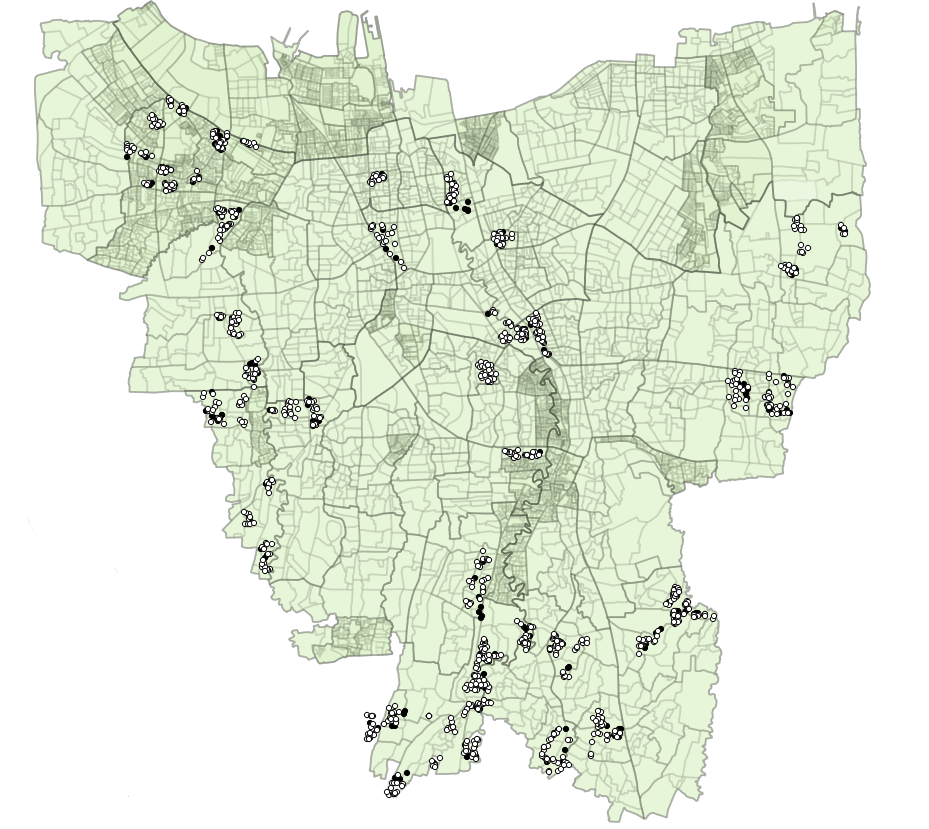
\includegraphics[width=120mm]{FigmapTC.png}
\end{figure}


\begin{figure}[h!]
    \centering
    \caption{Treatment Distribution across Retailers: Village Pegangsaan}
   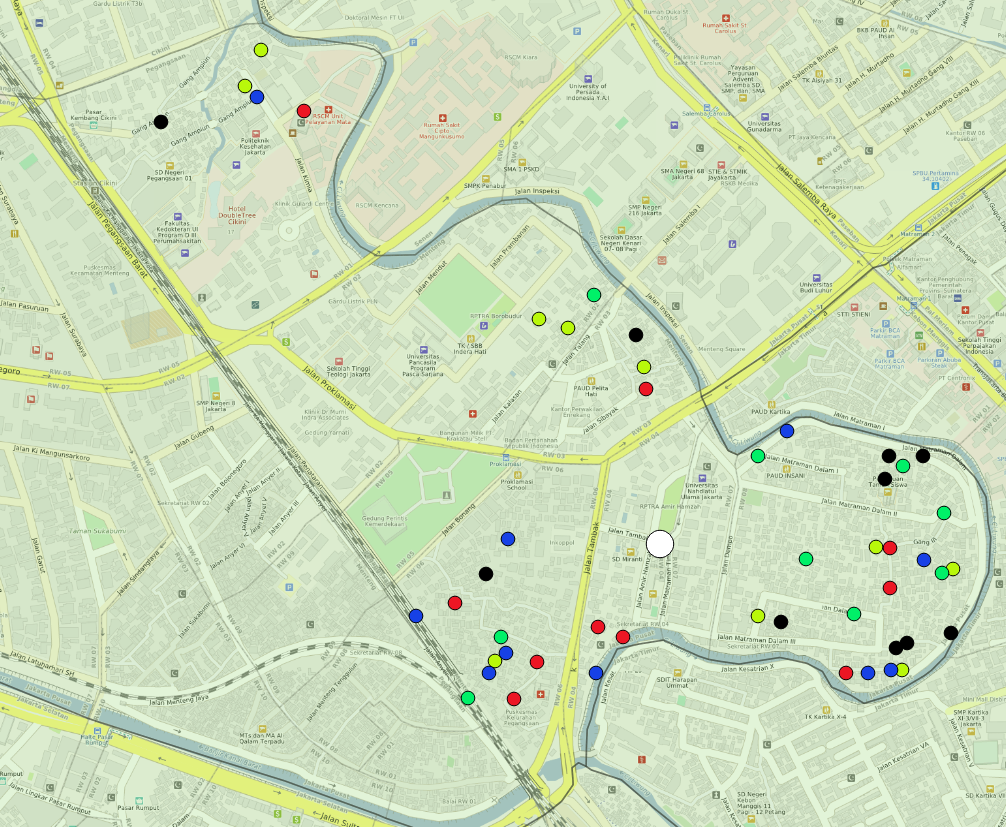
\includegraphics[width=120mm]{FigmapZoom.png}
\end{figure}


\pagebreak

\begin{figure}[h!]
    \centering
    \caption{Movie Screening Locations (big white) and Firms invited to the movie}
   	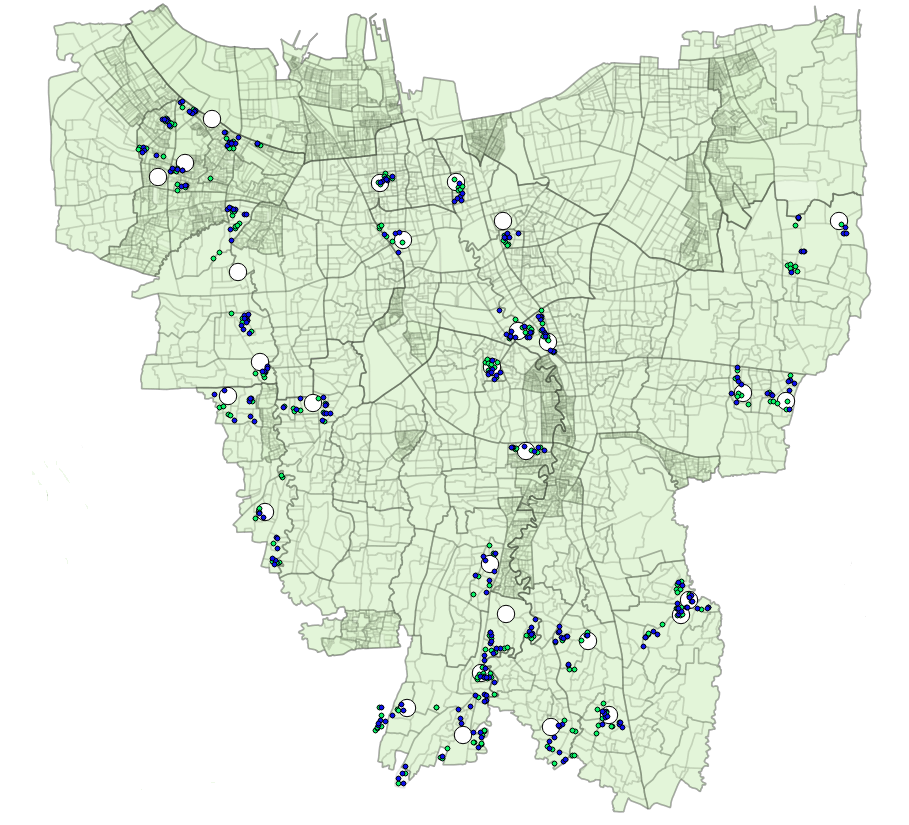
\includegraphics[width=120mm]{FigmapMovie.png}
\end{figure}

\end{landscape}
\pagebreak


\section{Sampling Protocol} \label{sec:appendixd}
\begin{enumerate}

	\item In the order given by the randomized list of selected villages, move 					into a village by approaching the respective head of the village.

	\item Obtain a list of all communities within the respective village and their 				boundaries.
	
	\item Generate a second list that contains these communities in random order.

	\item Move into a village according to the randomized list and, within each 				village, approach the owner of every shop that satisfies the following 				criteria:

	\begin{enumerate}
	
		\item The shop is at a distance of at least 30 meters to any other shop 					already listed.

		\item The shop is not a mere handcart or not otherwise easily moved.

		\item The shop is at least 4 $m^2$ in size

		\item The shop offers products from at least 2 product categories out of 					the following list:

		\begin{enumerate}


			\item Perishables (vegetables, fruits, eggs, rice, etc.)
			\item Pre-packaged food
			\item Soft-drinks and packaged drinks
			\item Snacks
			\item Tobacco
			\item Medicine
			\item Cleaning products
			\item Personal care
			\item DIY products

		\end{enumerate}

		\item The shop owner professes an aspiration to grow their business.

	\end{enumerate}

	\item Conditional upon the shop owner consenting, conduct the interview.

	\item Within the respective community, continue interviewing the owners of all 				shops that satisfy above mentioned criteria.

	\item If at any time the number of shops interviewed within the respective 					village equals or exceeds 67, continue interviewing all shops within 				the communities already moved into, but do not begin sampling in any 				new community within that village.

	\item If and when the total number of shops interviewed equals or exceeds 					2000, continue interviewing all shops within the village until the 					number of shops interviewed within the respective village equals or 				exceeds 67, in which case you continue interviewing all shops within 				the communities already moved into, but do not move into any new 					community within that village (just as outlined above).

\end{enumerate}
\pagebreak
\section{Project Timeline} \label{sec.timeline}

\begin{figure}[h]
    \centering
    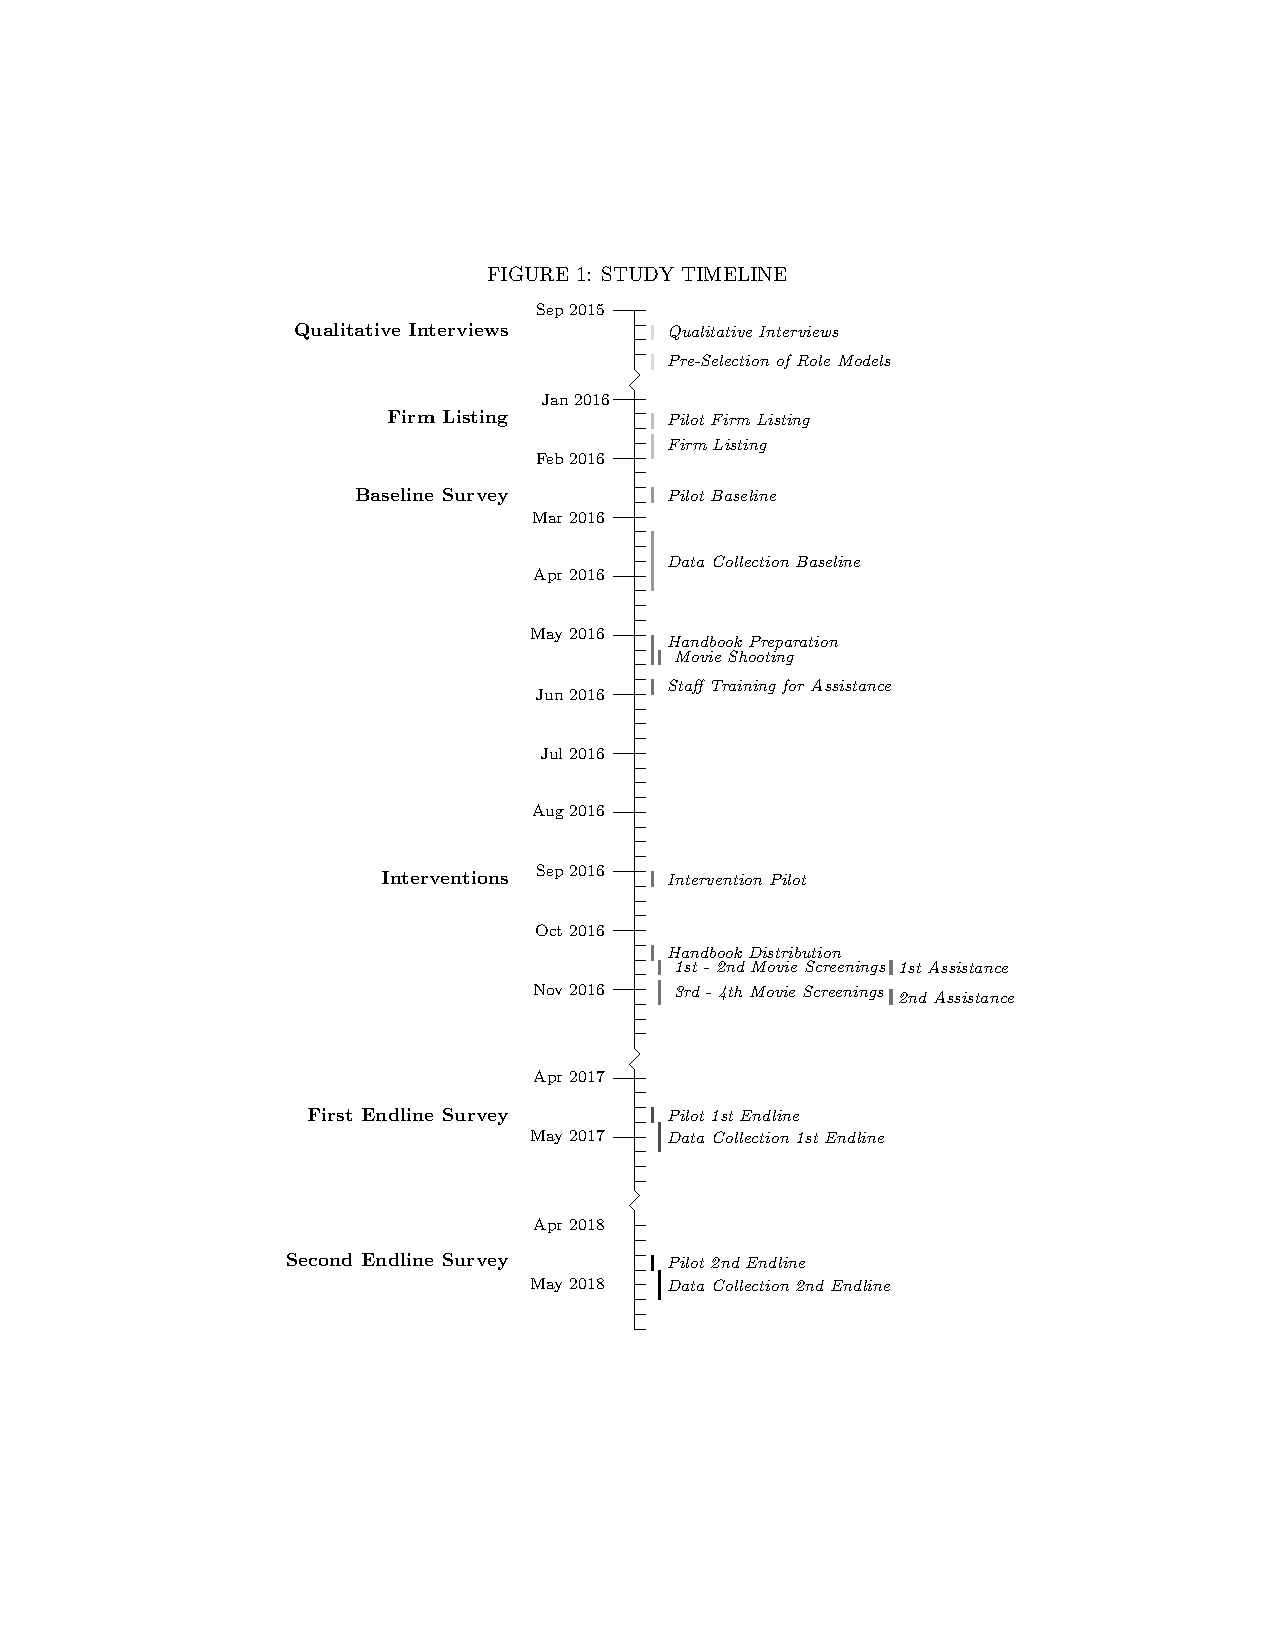
\includepdf[pages=-]{FigTimeline.pdf}
\end{figure}

\pagebreak
\section{Experimental Design} \label{sec:design}

\begin{table}[h!]
  \centering
  \renewcommand{\arraystretch}{1.4}
  \begin{tabular}{|c|c|c|c|c|c|c|c|c|}
    \hline
    \multicolumn{9}{|c|}{\textbf{Total Sample}}\\
    \multicolumn{9}{|c|}{1301 firms}\\
    \hline
    \multicolumn{1}{|c}{\textbf{Control}} & \multicolumn{8}{|c|}{\textbf{Handbooks}}\\
    \multicolumn{1}{|c}{261 firms} & \multicolumn{8}{|c|}{1040 firms}\\
    \cline{2-9}
    \multicolumn{1}{|c}{} & \multicolumn{8}{|c|}{\textbf{Returns to Adoption Framing}}\\
    \cline{2-9}
    \multicolumn{1}{|c}{} & \multicolumn{4}{|c}{\textit{Positive}} & \multicolumn{4}{|c|}{\textit{Negative}}\\
    \multicolumn{1}{|c}{} & \multicolumn{4}{|c}{520 firms} & \multicolumn{4}{|c|}{520 firms}\\
    \cline{2-9}
    \multicolumn{1}{|c}{} & \multicolumn{8}{|c|}{\textbf{Role Model Movie}}\\
    \cline{2-9}
    \multicolumn{1}{|c}{} & \multicolumn{2}{|c}{\textit{Yes}} & \multicolumn{2}{|c}{\textit{No}} & \multicolumn{2}{|c}{\textit{Yes}} & \multicolumn{2}{|c|}{\textit{No}}\\
    \multicolumn{1}{|c}{} & \multicolumn{2}{|c}{260 firms} & \multicolumn{2}{|c}{260 firms} & \multicolumn{2}{|c}{260 firms} & \multicolumn{2}{|c|}{260 firms}\\
    \cline{2-9}
    \multicolumn{1}{|c}{} & \multicolumn{8}{|c|}{\textbf{Counseling Assistance}}\\
    \cline{2-9}
    \multicolumn{1}{|c}{} & \multicolumn{1}{|c}{\textit{Yes}} & \multicolumn{1}{|c}{\textit{No}} & \multicolumn{1}{|c}{\textit{Yes}} & \multicolumn{1}{|c}{\textit{No}} & \multicolumn{1}{|c}{\textit{Yes}} & \multicolumn{1}{|c}{\textit{No}} & \multicolumn{1}{|c}{\textit{Yes}} & \multicolumn{1}{|c|}{\textit{No}}\\
	\multicolumn{1}{|c}{} & \multicolumn{1}{|c}{130} & \multicolumn{1}{|c}{130} & \multicolumn{1}{|c}{130} & \multicolumn{1}{|c}{130} & \multicolumn{1}{|c}{130} & \multicolumn{1}{|c}{130} & \multicolumn{1}{|c}{130} & \multicolumn{1}{|c|}{130}\\
	\multicolumn{1}{|c}{} & \multicolumn{1}{|c}{firms} & \multicolumn{1}{|c}{firms} & \multicolumn{1}{|c}{firms} & \multicolumn{1}{|c}{firms} & \multicolumn{1}{|c}{firms} & \multicolumn{1}{|c}{firms} & \multicolumn{1}{|c}{firms} & \multicolumn{1}{|c|}{firms}\\
	\hline
  \end{tabular}
\end{table}



\pagebreak
%\section{Selection of Role Models}\label{sec:rolemodel}

%\pagebreak
%\section{Movie Script}\label{sec:movie}

%Available upon request.


\section{Businesses Pictures}\label{sec:expbusinesses}

\begin{figure}[h!]
\centering
\caption{Pictures of two shops representative of the sample of small-scale retail businesses in this study}
\label{warung1}
    \includegraphics[width=120mm]{Warung1.jpg}
\end{figure}

\begin{figure}[h!]
\centering
\label{warung2}
    \includegraphics[width=120mm]{Warung2.png}
\end{figure}

\end{appendices}
\end{document} 